\documentclass{article}

\usepackage[utf8]{inputenc} % allow utf-8 input
\usepackage[T1]{fontenc}    % use 8-bit T1 fonts
\usepackage{hyperref}       % hyperlinks
\usepackage{url}            % simple URL typesetting
\usepackage{booktabs}       % professional-quality tables
\usepackage{amsfonts}       % blackboard math symbols
\usepackage{nicefrac}       % compact symbols for 1/2, etc.
\usepackage{microtype}      % microtypography
\usepackage{graphicx}
\usepackage{cite}
\usepackage{xcolor}
\usepackage{listings}
\lstset{basicstyle=\ttfamily,
    showstringspaces=false,
    commentstyle=\color{red},
    keywordstyle=\color{blue}
}


\title{DeepSV: a deep learning based variant scorer}

\author{
  Félix Raimundo\\
  Department of Computer Science\\
  École Polytechnique\\
  Palaiseau, France\\
  \texttt{felix.raimundo@inria.fr}
  %% examples of more authors
  %% \And
  %% Coauthor \\
  %% Affiliation \\
  %% Address \\
  %% \texttt{email} \\
  %% \AND
  %% Coauthor \\
  %% Affiliation \\
  %% Address \\
  %% \texttt{email} \\
  %% \And
  %% Coauthor \\
  %% Affiliation \\
  %% Address \\
  %% \texttt{email} \\
  %% \And
  %% Coauthor \\
  %% Affiliation \\
  %% Address \\
  %% \texttt{email} \\
}

\begin{document}

\maketitle

\begin{abstract}
  In this paper, we present DeepSV, a deep learning based method for scoring the likelihood that a set of anomalous read pairs are caused by a structural variant, by opposition to mapping or sequencing errors.
  
  We identified a region of fixed size that contains enough signal to make classification
  with deep learning methods, and thus allowing us to move away from the previous methods
  based on linear classifiers applied on few hand-crafted features.
\end{abstract}

\section{Definitions}

In this papers we will be using the sequencing terms as defined in \cite{li_sequence_2009}, whose most
relevant ones are copied here.

\paragraph{Segment} A contiguous sequence or subsequence.
\paragraph{Read} A raw sequence of DNA that comes off a sequencing machine.
\paragraph{Coverage} Number of reads mapped at a specific location in the reference genome.
\paragraph{Read Pair} Long sequence of DNA of which the sequencing machine reads the two extremities. Each of the extremities are reads, are associated a direction, and are separated by a distance called insert size.

Note: For the duration of this paper, we will assume that the two reads of a read pair are both directed to the center, i.e. the first read is directed from left to right, called forward, and the second right to left, called backward.

\section{Properties of the data}

In this paper we will be making the following two assumptions:

\paragraph{Assumption 1} The distance between two reads of a read pair, called insert size, follows a normal distribution when they are generated.
\paragraph{Assumption 2} The length of reads, called read size, follows a normal distribution.\\
Note: Empirical data is known not to verify theses assumptions, however they are a good approximation of reality and are used in most other variant callers (see \cite{ rausch_delly:_2012}, \cite{ye_pindel:_2009}, \cite{chen_manta:_2016}, \cite{handsaker_large_2015}, \cite{chen_breakdancer:_2009}).\\
Note: The distance between two reads of a pair generated from a target genome can be different once the two reads are mapped on a reference genome, the analysis of that phenomenon is the basis of our study.

\paragraph{Simplification 1} During the rest of this document we will assume that the insert size and read size are constant when the reads are generated, indeed the two distribution have a low standard deviation relative to the mean, this approximation is thus sensible.\\
All the future claims stay valid without this approximation, but would make the text much less readable by introducing many confidence intervals.

Section \emph{Dealing with reality} will describe how we deal with real data, where these assumptions are not correct.

\paragraph{Property 1} Because of assumptions 1 and 2, and simplification 1, it follows that the second pair of a read pair is fully contained within $[insert\_size, insert\_size + read\_size]$ of the end of the first one in the genome from which the reads are extracted.

\subsection{Structural Variants}

\paragraph{Variant} We call variant, a difference between the genome of the person being sequenced and the reference genome, they are the cause of the genetic diversity in the population.

Some variants are called \emph{structural variants}, because they are considered so large that they come from a structural difference. The limit between regular variant and structural variant does not have a proper definition, but they are usually considered to be changes affecting more than 50bp.

Structural variants are separated in two categories:
\begin{itemize}
    \item Balanced rearrangements: which do not affect the total number of nucleotides in the genome.
    \item Imbalanced rearrangements: which affect the total number of nucleotides in the genome, also called Copy Number Variation (CNV).
\end{itemize}

The CNVs are themselves divided in three categories:
\begin{itemize}
    \item Deletions: where a large portion of the genome is deleted relative to the reference.
    \item Tandem duplication: where a large portion of the genome is duplicated, potentially multiple times; the duplicates are directly next to each other.
    \item Interspersed duplication: where a large portion of the genome is duplicated, potentially multiple times;
    the duplicates are separated by segments of DNA.
\end{itemize}

Likewise the balanced rearrangements are divided in two categories:
\begin{itemize}
    \item Translocation: where a large portion of DNA is moved to another location in the genome (potentially on another chromosome).
    \item Inversion: where a large portion of DNA has the order of its nucleotides reversed.
\end{itemize}

In our study we will only work on deletions, tandem duplications, and inversions. We however believe that our method could be extended to work on the other types of variants (see \emph{Future Work}).

\paragraph{Breakpoint} We call breakpoints the locations where structural rearrangements happen in the genome being sequenced, there are:
\begin{itemize}
    \item 1 in the case of deletions.
    \item $n$ for tandem duplications with $n$ duplicates.
    \item $n$ for interspersed duplications with $n$ duplicates.
    \item 2 for inversions
    \item 2 for translocations.
\end{itemize}

\subsection{Methods of detection}

The current state of the art algorithms for finding structural variants are based on a mixture of the four following methods (see \cite{lin_making_2015} or \cite{sudmant_integrated_2015} for a deeper review):

\begin{itemize}
	\item Assembly based (AS), does \emph{de novo} assembly on regions suspected to contain an SV. They are rarely used as: assembly is computationally expensive and not always possible in regions with repetitive sequences.
	\item Read count (RC), observes the distribution of coverage in the genome. It can only detect CNVs as reads in translocations and inverted regions are properly mapped. Furthermore reads are not generated uniformly in the genome from which the reads come, it is thus not an optimal method alone.
	\item Split reads (SR), uses reads that fall on the breakpoint. Those reads are unmapped, as part of them is in the rearrangement. These reads are split so that they can be mapped properly. As the split reads are smaller than regular reads they cannot always be mapped unambiguously.
	\item Paired reads (PR), uses pairs of mapped reads that have an insert size far away from the mean insert size, or who do not have the expected orientation. This method is often used to identify regions that contain SV and followed by a finer analysis.
\end{itemize}

In the case of DeepSV we use paired reads to identify regions of interest and use a pattern recognition model on the selected regions to decide whether they contain an SV.
We expect our model to use RC and PR methods for predictions. AS and SR methods can be used to locate the breakpoints with higher precision once the prediction is made.

The next sections will explain what patterns we expect to find in these regions.

\subsection{Anomalous paired reads}

Anomalous read pairs (ARP) are read pairs that do not have the normal orientation or insert size once mapped.

\paragraph{Property 2}  Assuming no errors in the reads or mapping, ARPs contain a breakpoint between their two reads.

Indeed, if one read was on the breakpoint, it could not be mapped as a part of it would be on a large rearrangement.

Respectively, if both reads were the same side of a  breakpoint, they would be mapped normally and would
thus not be caught as anomalous.

\paragraph{Property 3} Because of properties 1 and 2 we can conclude that all reads in ARPs will be at most $read\_size + insert\_size$ away from the breakpoint in the genome that generated the reads.

\subsubsection{Deletion}

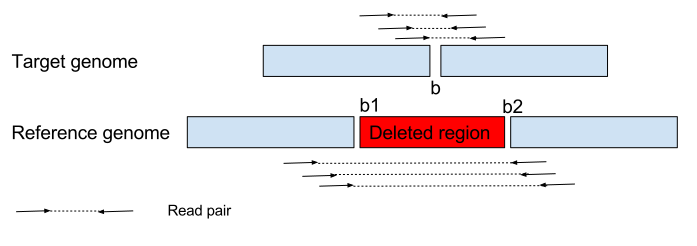
\includegraphics[width=\textwidth]{DeletionReadPairs}

In the case of deletions there is a single breakpoint $b$, the deleted region is $[b1, b2]$.

Assuming no errors in the reads or mapping:
\begin{itemize}
    \item reads originally left of $k$bp from b will be mapped at $[b1 - k - read\_size, b1 - k]$ instead of $[b - k - read\_size, b - k]$ and in the correct direction.
    \item reads originally right of $k$bp from b will be mapped at $[b2 + k, b2 + k + read\_size]$ instead of $[b + k, b + k + read\_size]$ and in the correct direction.
    \item no reads should be mapped in $[b1, b2]$.
\end{itemize}

In the case of ARPs, by using property 3, we know that $k < insert\_size$, we can thus conclude that all ARPs will be contained within $[b1 - insert\_size - read\_size, b1] \cup [b2 + insert\_size + read\_size, b2]$,
these reads will have an expected distance of $insert\_size + (b2 - b1)$.

By using property 3, we can conclude that given a set of ARPs supporting a deletion, b1 will be contained within $insert\_size + read\_size$ of the leftmost read, and b2 will be contained within $insert\_size + read\_size$ of the rightmost read.

We have thus constructed two intervals containing all the ARPs and RC information, these two intervals' sizes are only dependent on the insert size and read size, not the size of the deletion. 

\subsubsection{Inversion} 

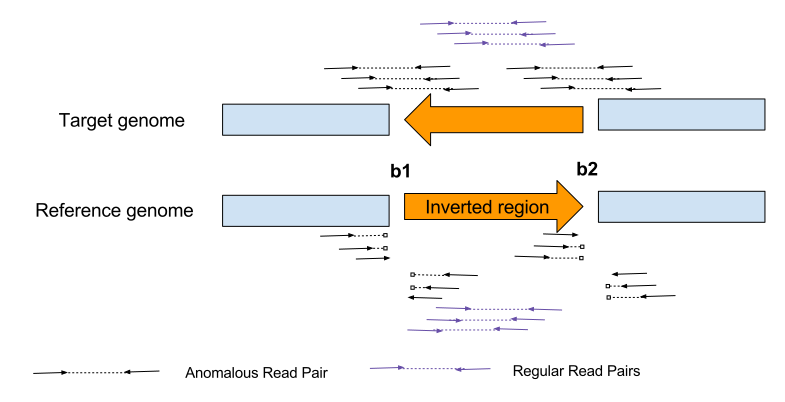
\includegraphics[width=\textwidth]{InversionReadPairs}

In the case of inversions there are two breakpoints b1 and b2, the inverted region is $[b1, b2]$.\\
ARPs will be read pairs with one read to the left of b1 and the other in the inverted region, or read pairs with one read to the right of b2 and the other in the inverted region.

Assuming no errors in the reads or mapping:
\begin{itemize}
    \item reads originally right of $k$bp from b1 will be mapped at $[b2 - k - read\_size, b2 - k]$ instead of $[b1 + k, b1 + k + read\_size]$ and in the opposite direction.
    \item reads originally left of $k$bp from b2 will be mapped at $[b1 + k, b1 + k + read\_size]$ instead of $[b2 - k - read\_size, b2 - k]$ and in the opposite direction.
    \item there is no variation in coverage, except at the breakpoints were the reads will not be mapped.
\end{itemize}


In the case of ARPs, by using property 3, we know that $k < insert\_size$, we can thus conclude that all ARPs will be contained within $[b1 - insert\_size - read\_size, b1 + insert\_size + read\_size] \cup [b2 - insert\_size - read\_size, b2 + insert\_size + read\_size]$

By using property 3, we can conclude that given a set of ARPs supporting an inversion, b1 will be contained within $insert\_size + read\_size$ of the leftmost read, and b2 will be contained within $insert\_size + read\_size$ of the rightmost read.

We have thus constructed two intervals containing all the ARPs and RC information, these two intervals' sizes are only dependent on the insert size and read size, not the size of the inversion. 

Note: This only works for inversions larger than $insert\_size + read\_size$.

\subsubsection{Tandem Duplication}

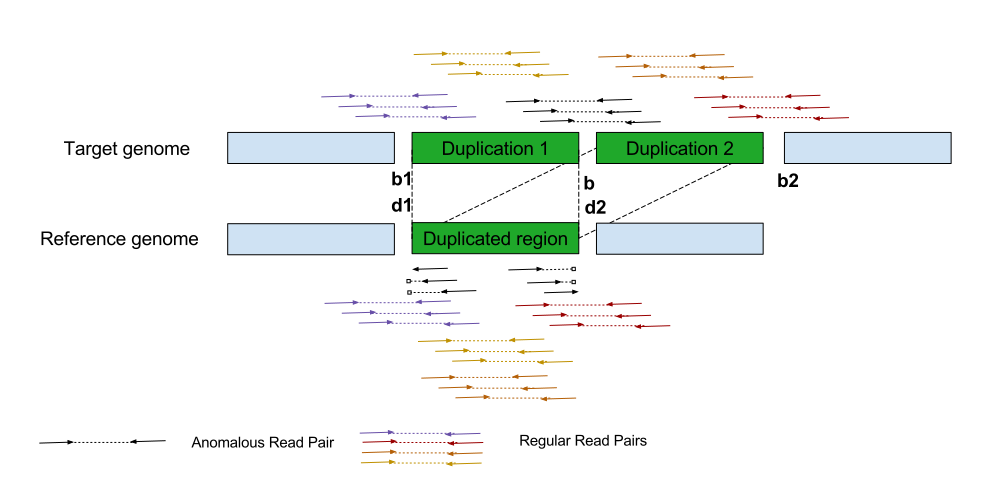
\includegraphics[width=\textwidth]{DuplicationReadPairs}

In the case of a tandem duplication with n duplicates, there are n breakpoints $b^1$,...,$b^n$, the duplicated region is $[d1, d2]$. The breakpoints are at the junction between duplicates.\\
Note: For the sake of clarity there is only one duplicate in the figure.

In the case of tandem duplications, the ARPs are read pairs with, with $i\in[1, n]$, have one read left of $b^i$ and one read right of $b^i$.

Assuming no errors in the reads or mapping:
\begin{itemize}
    \item reads originally left of $k$bp from $b^i$ will be mapped at $[d2 - k - read\_size, d2 - k]$ instead of $[b^i - k - read\_size, b^i - k]$ and in the correct direction.
    \item reads originally right of $k$bp from $b^i$ will be mapped at $[d1 + k, d1 + k + read\_size]$ instead of $[d^i + k, d^i + k + read\_size]$ and in the correct direction.
    \item ARPs will thus have the order of their reads reversed, both reads will thus have opposite direction relative to normal read pairs.
    \item coverage in $[d1, d2]$ is expected to be $1 + n$ times higher than in non duplicated areas.
\end{itemize}

In the case of ARPs, by using property 3, we know that $k < insert\_size$, we can thus conclude that all ARPs will be contained within $[d1, d1 + insert\_size + read\_size] \cup [d2, d2 + insert\_size + read\_size]$, coverage in that region will be $1 + n$ times higher than in non duplicated areas.

By using property 3, we can conclude that given a set of ARPs supporting a tandem duplication, d1 will be contained within $insert\_size$ of the leftmost read, and d2 will be contained within $insert\_size$ of the rightmost read.

We have thus constructed two intervals containing all the ARPs and RC information, these two intervals' sizes are only dependent on the insert size and read size, not the size of the duplicated area northe number of duplicated. 

Note: This only works for duplicates larger than $insert\_size + read\_size$.

\subsection{Conclusion}

We have shown that, given a variant and its breakpoints, we can construct two windows of size $2 \times (insert\_size + read_size)$ each, centered on the two boundaries in the reference genome, that contains all the ARPs that support it.\\

We have also shown that given a type of variant and ARPs supporting it, we can locate two intervals containing the boundaries, and from there two windows containing all the ARPs that would support that variant.

The size of these windows are only dependent on the $insert\_size$ and $read\_size$, not on the size of the structural rearrangements.

It is noteworthy that both $insert\_size$ and $read\_size$ will be extremely close between individuals provided they are sequenced using the same protocol. Our method will thus be able to predict variants on all future individuals sequenced using the same protocol. TODO CITATION.

By taking the largest intervals of the three sub sections above, we can have a single model that will deal with all variants (except for translocations and interspersed duplications).

\subsection{Future works}

In this work we presented an algorithm for scoring the likelihood that a region contains a structural variant, by extracting a intervals independent on the size of the variants and using pattern matching models from the deep learning community.\\
However this algorithm is not sufficient for finding variants from raw reads, we plan on integrating this algorithm in a full variant discovery pipeline that would emit the candidates variants as well as refining the location of the breakpoints.This full pipeline will be released with an open source license in the months following the publication of this paper.

We chose not to deal with translocations and interspersed duplications in this work is because they would require to consider twice as much intervals and we have not found an elegant way to use the same model for them. However we could very well have a model for [deletion, tandem duplication, inversion] and a model for [translocation, interspersed duplication].

\section{Dealing with real data}

As said before, the empirical insert size does not follow a normal distribution. We can see that it is skewed towards lower values. However, we can see that the distribution is well centered on its mean: 400 bp.

\includegraphics[width=\textwidth]{insert_size_histogram}

\begin{lstlisting}[language=bash,caption={Picard command}]
#!/bin/bash
java -jar picard.jar CollectInsertSizeMetrics \
    I=input.bam \
    O=insert_size_metrics.txt \
    H=insert_size_histogram.pdf \
    M=0.5
\end{lstlisting}

We are aware of two reasons that could cause such a skew:
\begin{itemize}
    \item Mobile element insertions of ALUs.
    \item Poor mapping in ambiguous regions.
\end{itemize}

Picard tells us that a width of 165 centered on the median, 386bp, will catch 95\% of the reads,
which will be considered a sufficient approximation. In consequence when building our window we will
consider an insert size of 467bp.

\section*{References}

\bibliography{deepSVbib.bib}{}
\bibliographystyle{unsrt}

\end{document}